%%%%%%%%%%%%%%%%%%%%%%%%%%%%%%%%%%%%%%%%%%%%%%%%%%%%%%%%%%%%%%%%%%%%%%%%%%%%%%%

% exemplo figura
\begin{figure}[!ht]
    \centering
    \caption{Comparison of Storm Tracks Across All 16 Experiments} % Título acima da figura
    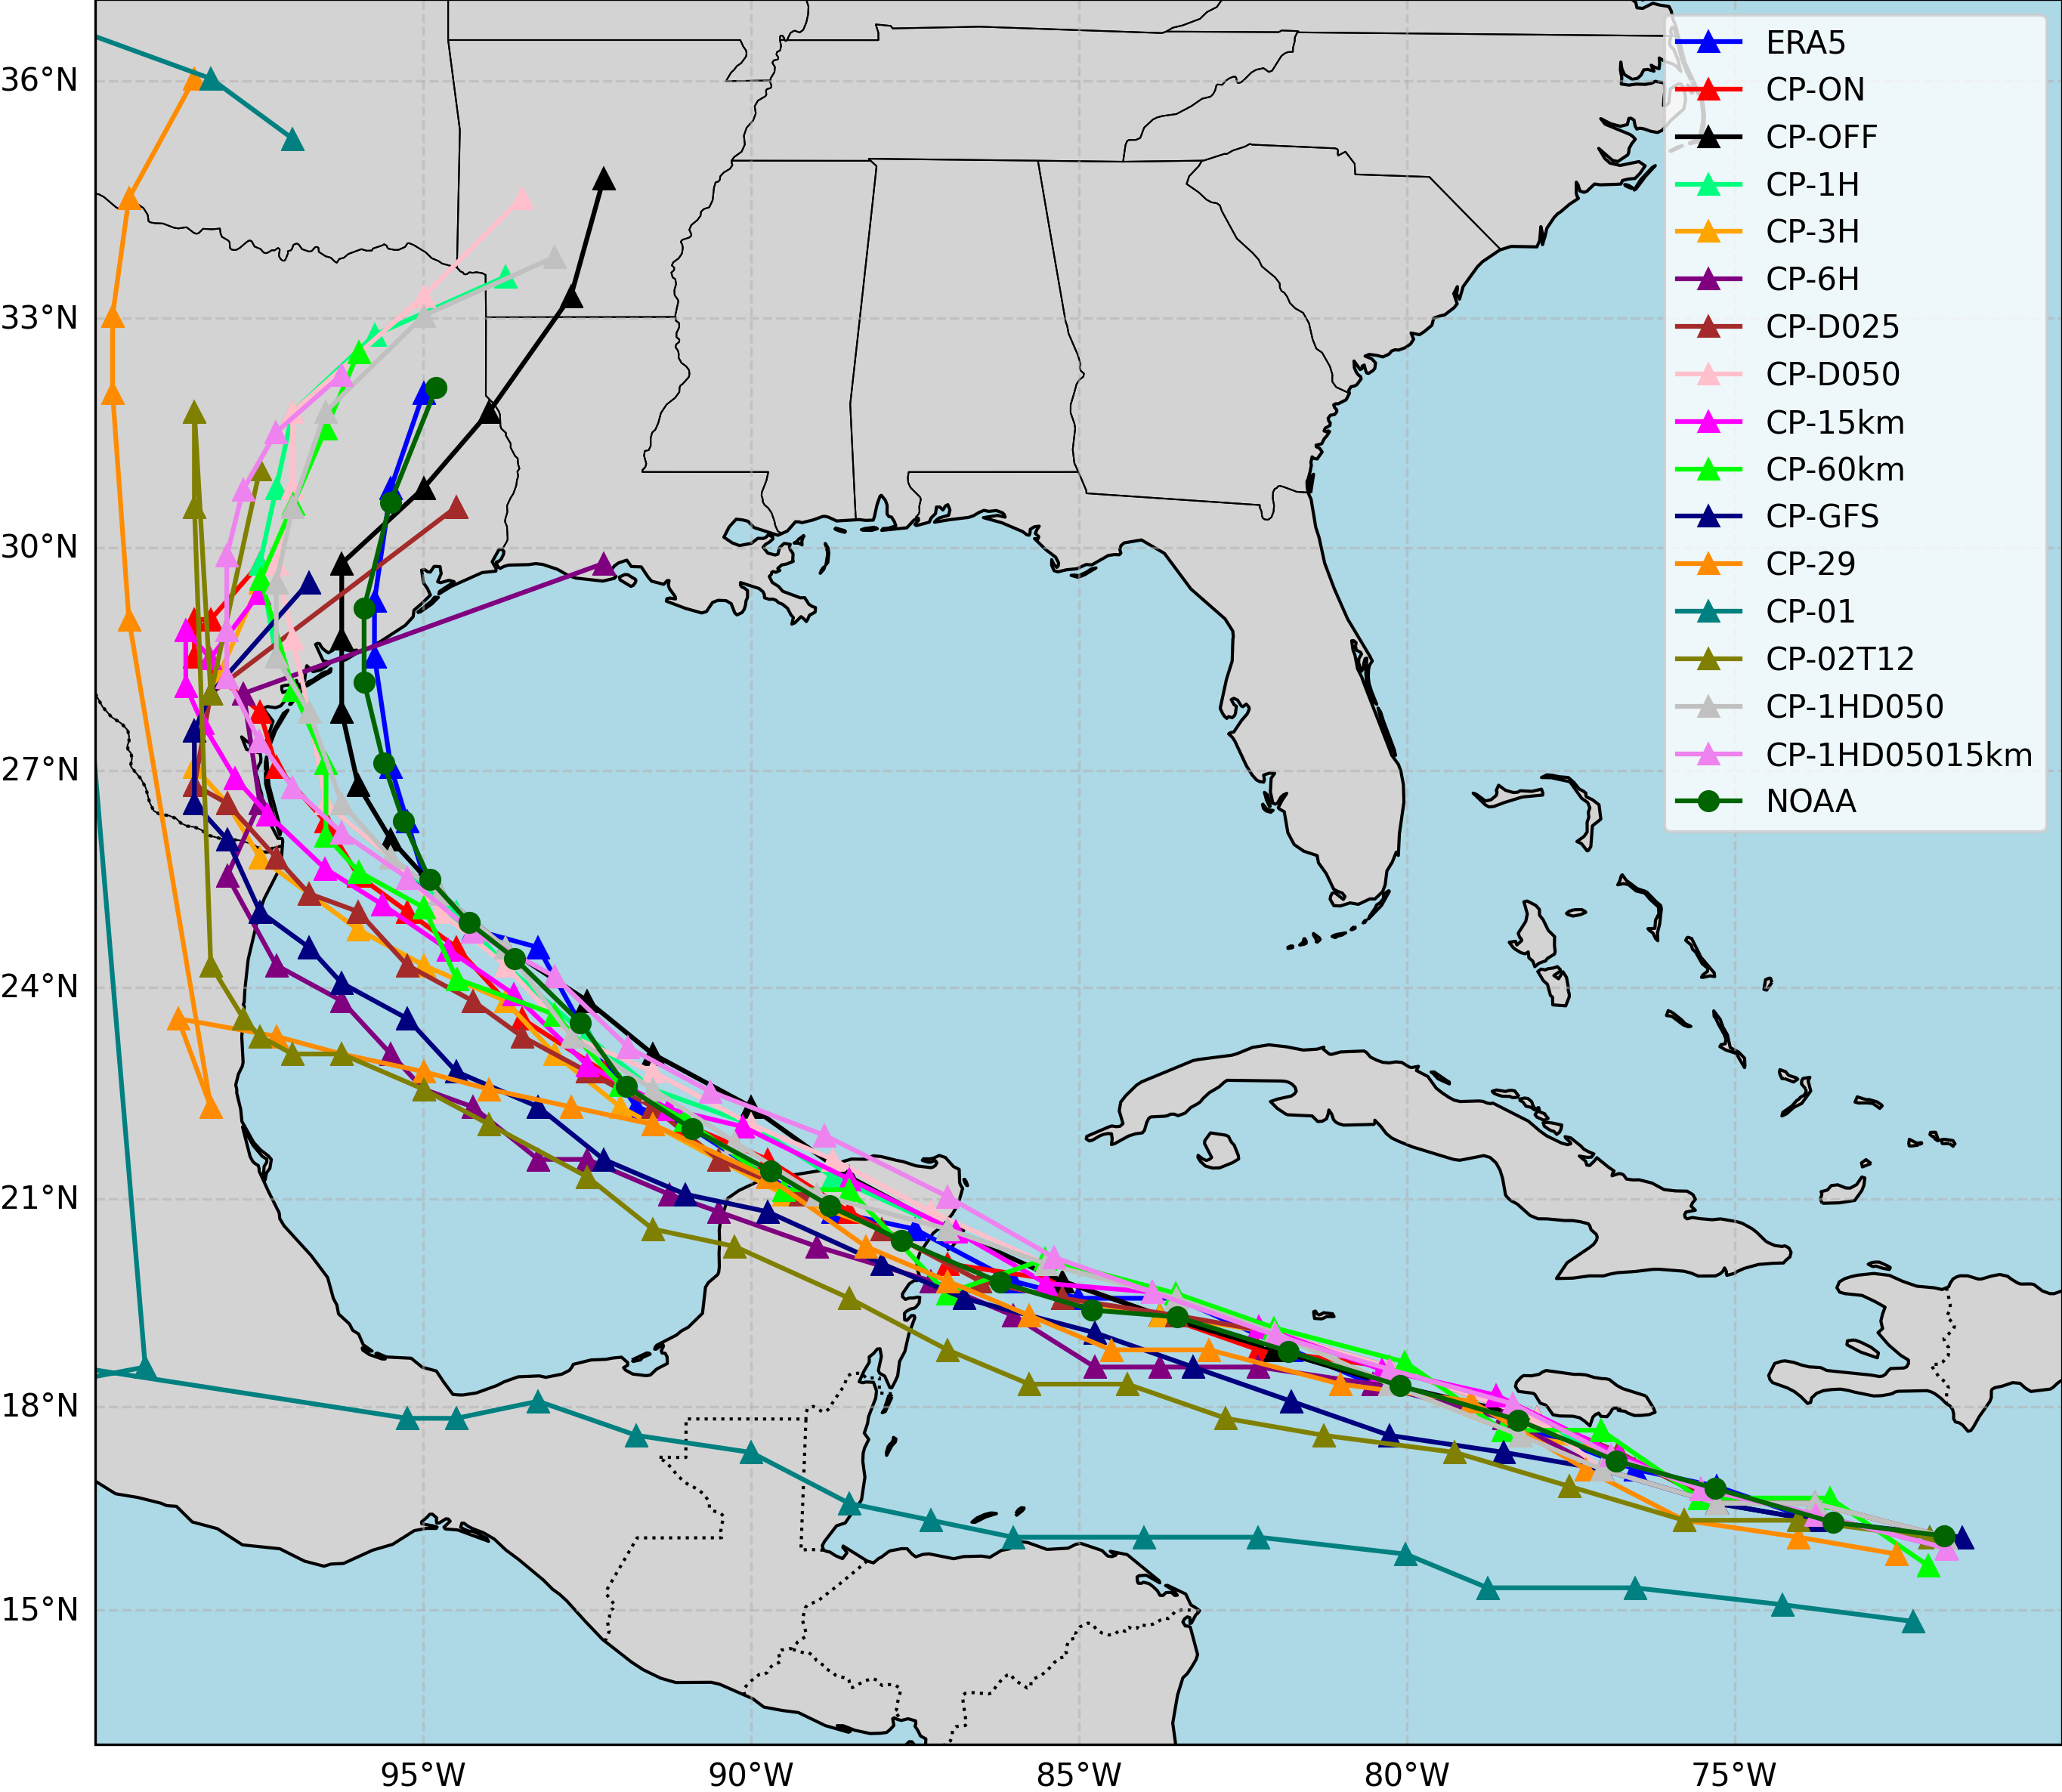
\includegraphics[width=\textwidth]{docs/figuras/findings/ALL_tracks.png} % Substitua pelo caminho e extensão correta
    \vspace{0.5em}
    
    Source: Made by the author (2025). % Fonte abaixo da imagem
    \label{fig:all_tracks_before} % Label para referenciar no texto
\end{figure}


\chapter{INTRODUÇÃO}

\citeonline{Cloude1996} menciona que complexidade da turbulência tem atraído \cite{Chelimsky2010, Chelimsky2010XX} a atenção de naturalistas, filósofos, e poetas durante vários séculos. Talvez o primeiro esboço de um fluxo turbulento, capturando detalhes com vários graus de realismo, tenha sido feito ainda no século XV por Leonardo da Vinci~\cite{sreenivasan/99}. Desde então, estudos científicos intensos em turbulência têm sido realizados, porém os resultados obtidos ainda não têm recompensado os grandes esforços empregados. Diversos modelos propostos ao longo do tempo, que incluem aqueles introduzidos por Kolmogorov e Landau deixam a desejar na descrição, explicação e predição do movimento turbulento~\cite{ruelle/91}. Conseqüentemente, a turbulência, durante o último século, foi considerada um dos problemas mais ``intratáveis'' da Física Clássica. Em resposta a essas dificuldades, novos modelos para o problema surgiram recentemente, influenciados pelo advento da teoria do caos, em particular através da caracterização via ``atratores caóticos''~\cite{ruelltak/71} 

O artigo clássico de \citeonline{lor/63} foi um dos primeiros trabalhos a descrever movimentos caóticos sobre um atrator de baixa dimensão. Tais movimentos são caracterizados por uma instabilidade intrínseca devido à sensibilidade do sistema às variações de suas condições iniciais. Como conseqüência, trajetórias de pontos inicialmente muito próximos separam-se, em média, exponencialmente ao longo do tempo no espaço de fase. É bastante surpreendente que um sistema dinâmico de apenas três dimensões, ou seja, descrito por três equações diferenciais ordinárias de primeira ordem, exiba movimentos surpreendentemente complexos que se assemelham, a primeira vista, a uma evolução aleatória. Desde que Lorenz introduziu seu modelo como uma aproximação da dinâmica de uma camada de fluido convectiva, conjectura-se que a atmosfera possa ter um intrínseco limite de previsibilidade e que a dinâmica atmosférica possa ser governada por atratores caóticos~\cite{weber/95}. 

Diversos estudos confirmam a presença de atratores caóticos associados a situações específicas, a partir de séries temporais em diferentes áreas. Porém, a existência ou não desses atratores ainda é um tema controverso. Atratores caóticos de baixa dimensão têm sido encontrados em trajetórias de ciclones tropicais~\cite{fraedrichandleslie/89}, em séries temporais marítimas~\cite{fraedrich/86,nicolis/84}, como também em séries temporais relacionadas ao fenômeno El Niño~\cite{goberelnino/92}. Atratores similares foram também encontrados na camada limite atmosférica a partir de séries temporais de pressão de superfície~\cite{fraedrich/86}, como também em séries temporais de temperatura, velocidade e umidade~\cite{xin/01,jaramillo/93,gallego/01,tiong/93}. Ainda, atratores de alta dimensão têm sido encontrados por \citeonline{grass/86} a partir de séries marítimas. Por outro lado, nenhum indício de um atrator foi encontrado nas análises realizadas por \citeonline{weber/95} com base em séries temporais turbulentas da velocidade do vento. Aliás, \citeonline{loratrat/91} afirma que não há razão alguma para acreditar que um sistema dinâmico complexo, como o clima, possua um atrator caótico de baixa dimensão associado. Ele conjecturou que a dinâmica caótica de baixa dimensão obtida por muitos autores, com base em séries temporais climáticas, está relacionada a existência de um conjunto de subsistemas de baixa dimensão ``fracamente'' acoplados ao sistema - clima.

A identificação de uma dinâmica caótica de baixa dimensão em escoamentos turbulentos na atmosfera tem permitido, se não conclusões definitivas, uma interpretação alternativa dos processos turbulentos, onde as estruturas dissipativas coerentes desempenham um papel relevante. Fisicamente, tais estruturas estão presentes nas grandes escalas do escoamento e podem agir como objetos rígidos descritos com poucos graus de liberdade. Desta forma, a detecção experimental de uma dinâmica de baixa dimensão pode estar relacionada não ao fenômeno da turbulência ``per se'', mas devido à existência de estruturas coerentes na atmosfera, como de certa forma intuído por \citeonline{loratrat/91}. Sob essa perspectiva, a complexidade da atmosfera que, a priori, deveria ser representada por um sistema dinâmico de alta dimensão, pode ``conter'' um ou mais atratores caóticos de baixa dimensão acoplados entre si.

%Contudo, é importante destacar que a compreensão física e matemática da \textit{turbulência completamente desenvolvida} como um fenômeno de alta dimensão, embora seja ainda incompleta, está em discordância com a figura de uma dinâmica de baixa dimensão que pode descrever vários aspectos da chamada \textit{turbulência fraca}~\cite{weber/95}. 

Estudos demonstram que a presença de estruturas coerentes em escoamentos turbulentos pode ser responsável, em média, por $40\%$ de todo o calor turbulento e fluxos de momento~\cite{lu/94}. Sob condições convectivas, elas são reconhecidas em séries temporais de flutuações de temperatura com uma gradual elevação da temperatura, seguida por uma súbita queda. Sob condições estáveis, este padrão se inverte e uma gradual queda é seguida por uma súbita elevação~\cite{oliver/02}. Nestas duas condições, a estrutura coerente é do tipo ``rampa''. 

A teoria de sistemas dinâmicos tem fornecido novas ferramentas para a análise de séries temporais estacionárias obtidas em experimentos, ou seja, com base na medida de um único observável $x(t_{i}),i=1,2,3,\ldots$. Pode até ser a única variável independente disponível associada ao sistema. Ou seja, é possível definir um espaço de fase que capture a dinâmica do sistema em uma estrutura geométrica imersa nesse espaço. O conjunto geométrico imerso é chamado \textit{atrator reconstruído} e ele é topologicamente equivalente ao atrator que seria produzido pela evolução do sistema dinâmico de equações, caso as mesmas fossem conhecidas. Reconstruída a dinâmica, a caracterização dos atratores pode ser feita por uma abordagem métrica. Esta abordagem, invariante por mudança de sistema de coordenadas, efetiva-se segundo uma \textit{caracterização dinâmica} ou então \textit{estático-estatística}. Na caracterização dinâmica obtém-se informações a respeito da taxa de expansão de trajetórias inicialmente próximas via expoentes de Lyapunov~\cite{eckrue/86,sanosawada/85} ou da taxa de produção de informação no sistema via entropia de Kolmogorov-Sinai~\cite{ruelleentrop/89}. Na caracterização estático-estatística, obtém-se informações sobre a estrutura local dos atratores, que se caóticos, serão, salvo raras exceções, caracterizados por uma medida fractal, que pode ser analisada através das dimensões generalizadas~\cite{grassproca/83}.

Existe à disposição uma grande variedade de algoritmos para a caracterização de caoticidade em baixa dimensão de sinais experimentais. Esses algoritmos, longe de constituir um corpo preciso, envolvendo na sua aplicação aspectos ainda não totalmente elucidados e estimativas de erro aparentemente otimistas, incluem procedimentos para a obtenção do espectro de expoentes de Lyapunov, da entropia de Kolmogorov-Sinai, da dimensão de correlação, etc. Ligada à caracterização de caos está a questão da redução de ruído e da reconstrução da dinâmica, problemas ainda não completamete resolvidos na análise de sinais experimentais~\cite{aguirre/00}. 

De modo geral, o objetivo deste trabalho é investigar a possível natureza caótica da turbulência na camada limite atmosférica, no interior e acima da copa da floresta Amazônica. Mais especificamente, deseja-se: (i) determinar se o conjunto de séries temporais em estudo inclui componentes com características de dinâmica caótica, que podem ser descritas (individualmente) por um sistema determinístico de baixa dimensão; (ii) compreender o papel das estruturas coerentes do tipo rampa na possível natureza caótica da turbulência sobre a copa da floresta Amazônica. Espera-se que os resultados aqui obtidos permitam elucidar a conjectura de \citeonline{loratrat/91}, partindo do pressuposto que os subsistemas atmosféricos de baixa dimensão, postulados por este autor, sejam de fato estruturas coerentes. Paralelamente, procura-se avaliar o desempenho de diversas ferramentas computacionais de caracterização de dinâmica caótica de baixa dimensão, na análise de séries temporais experimentais longas e contaminadas com ruído.

Neste trabalho, foram utilizados dados turbulentos de temperatura e velocidade do vento, obtidos pela campanha WETAMC (Campanha de Mesoescala Atmosférica na Estação Úmida) do projeto LBA (Experimento de Grande Escala de Interação Biosfera-Atmosfera na Amazônia), amostrados a $60$ Hz, com duração de $30$ minutos. As medidas foram feitas com o auxílio de uma torre micrometeorológica de $66$ m de altura, simultaneamente em três diferentes alturas: Nível Superior ($66$ m - acima da copa); Nível Médio ($45$ m -  no topo da copa); e Nível Inferior ($21$ m - abaixo da copa). Dois períodos de medidas distintos foram selecionados: às 12 horas, quando a copa da floresta é aquecida pelo sol e o topo da copa é mais quente que os arredores, e assim a região acima da copa é instável; e às 23 horas, quando as condições são opostas, e a região acima da copa é estável~\cite{Ramos/04}.

%Os capítulos restantes desta dissertação estão organizados da seguinte maneira:
%\begin{itemize}
%\item{Capítulo 2}: A Seção~\ref{seccaos} aborda, por meio de sistemas-paradigma de comportamento caótico como o Mapa Logístico e as Equações de Lorenz, as principais características apresentadas por sistemas dinâmicos não-lineares caóticos. A Seção~\ref{secturb} é destinada, em grande parte, à descrição fenomenológica da turbulência. São ainda apresentadas alguns temas de grande relevância no estudo da turbulência, como o fenômeno da intermitência e as estruturas coerentes. Finalmente, a Seção~\ref{seccaosurb} expõe uma perspectiva adicional para a compreensão do fenômeno turbulento com base na teoria de sistemas dinâmicos, mais especificamente por meio de atratores caóticos~\cite{ruelltak/71}.
%\item{Capítulo 3}: Neste capítulo é feita uma descrição detalhada dos métodos e dos algoritmos disponíveis para a caracterização de caos determinístico presente em séries temporais experimentais. O tema é bastante extenso e especializado; como conseqüência, tal descrição será focada nos procedimentos mais utilizados para a reconstrução da dinâmica, para o cálculo de dimensão de atratores e do espectro de expoentes de Lyapunov. São abordados alguns problemas e limitações, do ponto de vista numérico, associados aos algoritmos utilizados, como também as dificuldades encontradas no tratamento de sinais experimentais. 
%\item{Capítulo 4}: Neste capítulo é realizada uma breve descrição dos dados coletados pela campanha WETAMC do projeto LBA, bem como do sítio experimental.
%\item{Capítulo 5}: Neste capítulo são aplicadas diversas ferramentas (descritas no Capítulo~\ref{caputiltecnicas}) nas séries temporais em estudo, em busca de atratores caóticos de baixa dimensão na camada limite atmosférica.
%\item{Capítulo 6}: Com base nas análises realizadas no Capítulo~\ref{capanaliseseresults}, neste capítulo serão apresentadas as conclusões obtidas, como também algumas sugestões para trabalhos futuros.
%\end{itemize}

